\documentclass[conference]{IEEEtran}

\usepackage[T1]{fontenc}
\usepackage{amsmath,amssymb}
\usepackage{graphicx}
\usepackage{booktabs}
\usepackage{cite}
\usepackage{xcolor}
\usepackage{url}

\newcommand{\todo}[1]{\textcolor{red}{\textbf{[#1]}}}
\graphicspath{{../figures/}{../../results/figures/}}

\begin{document}

\title{Memory--Logic Trade-off of Full-Cycle and Quarter-Wave Sine ROMs\\
in a Fixed-Point AM Modulator on Artix-7}

\author{\IEEEauthorblockN{Pham Minh Tung, Mai The Tam, Cao Huu An, \todo{fourth member}}
\IEEEauthorblockA{FPT University\\
RTL Design Project\\
}}

\maketitle

\begin{abstract}
We present a fixed-point double-sideband full-carrier (DSB-FC) amplitude
modulator written in Verilog, in which two numerically controlled oscillators
(NCOs) generate the carrier and the message and two integer multipliers form
the modulated output. The design is verified bit-exactly against an
integer-only Python golden model over 13 configurations covering modulation
indices from 0 to 1.5, DSB-SC operation and a wider message bandwidth; no
sample of the 130\,000 compared differs. We then compare two sine-table
architectures, a full-cycle ROM and a quarter-wave ROM, for 8-, 10- and 12-bit
table addresses on an xc7a35tcpg236-1 device at 100~MHz. The two architectures
produce identical output at every address width, so the measured SFDR of 48.1,
60.7 and 71.9~dB depends only on the address width and follows
$6.02\,AW$~dB. The quarter-wave table stores 75\% fewer words;
\todo{measured LUT, BRAM and Fmax difference}.
All figures are reproducible from the repository with a single command.
\end{abstract}

\begin{IEEEkeywords}
amplitude modulation, direct digital synthesis, FPGA, quarter-wave ROM, fixed-point, Verilog
\end{IEEEkeywords}

\section{Introduction}
Amplitude modulation (AM) remains the simplest way to impress a low-rate
message on a high-frequency carrier, and its envelope-detectable waveform makes
it a convenient test case for digital transmitter design. In a digital
implementation the carrier and the message are produced by direct digital
synthesis (DDS)~\cite{tierney1971}: a phase accumulator addresses a sine table,
and the output frequency is set by a single tuning word, so the same hardware
serves any frequency without redesign.

The sine table dominates the memory cost of a DDS. Because a sine wave is
symmetric, storing one quarter of a period is enough to rebuild the whole
period, at the price of extra logic that mirrors the address and negates the
sign~\cite{nicholas1987,vankka2005}. Whether this saving pays off on an FPGA,
where small tables are mapped to distributed RAM and large ones to block RAM,
is not obvious in advance. This paper answers the question for a complete AM
modulator rather than for an isolated NCO.

The contributions are: (i) a parameterized Verilog AM modulator in which the
ROM architecture and the address width are the only design variables;
(ii) a bit-exact verification flow driven by an integer-only golden model and
spectral checks; and (iii) post-implementation resource, timing and power
figures for six ROM configurations, generated by a single script.

The scope is the modulator only. Demodulation is not implemented, and no
hardware board is used: all results come from simulation and from Vivado
synthesis and implementation targeting the xc7a35tcpg236-1 device.

\section{Theory}
\subsection{Amplitude modulation}
A DSB-FC AM signal is
\begin{equation}
s(t)=A_c\bigl[1+\mu\,m(t)\bigr]\cos(2\pi f_c t),\qquad |m(t)|\le 1,
\label{eq:am}
\end{equation}
where $f_c$ is the carrier frequency, $A_c$ the carrier amplitude and
$\mu=A_m/A_c$ the modulation index. For a single-tone message
$m(t)=\cos(2\pi f_m t)$, \eqref{eq:am} expands to
\begin{multline}
s(t)=A_c\cos(2\pi f_c t)+\tfrac{\mu A_c}{2}\cos\bigl(2\pi(f_c+f_m)t\bigr)\\
+\tfrac{\mu A_c}{2}\cos\bigl(2\pi(f_c-f_m)t\bigr),
\label{eq:lines}
\end{multline}
that is, exactly three spectral lines. The two sidebands are each $\mu/2$ of the
carrier ($-12.04$~dB for $\mu=0.5$), the occupied bandwidth is $B=2f_m$, and only a
fraction $\mu^2/(2+\mu^2)$ of the transmitted power carries the message~\cite{haykin2001}.

The envelope $A_c[1+\mu m(t)]$ stays positive only for $\mu\le1$. At $\mu=1$ it
touches zero (critical modulation), and for $\mu>1$ it changes sign, so an
envelope detector recovers a distorted message. This overmodulation is a
property of the receiver; the transmitted product in \eqref{eq:am} is still
linear, so its spectrum keeps three lines. Setting $A_c=0$ removes the carrier
line and gives DSB-SC, for which the sideband-to-carrier ratio is undefined.

\subsection{Fixed-point implementation}
Samples are signed integers in which $2047$ represents $1.0$. The product of two
such numbers carries the scale factor $2^{11}$ twice, so each multiplication is
followed by an arithmetic right shift of 11 bits:
\begin{align}
m_t &= (A_m\cdot m)\gg 11, & e &= A_c + m_t, & y &= (e\cdot c)\gg 11,
\label{eq:fixed}
\end{align}
with $m$ and $c$ the 12-bit message and carrier samples, $e$ a 14-bit envelope
and $y$ a 16-bit output. An arithmetic right shift rounds toward $-\infty$, which
the golden model reproduces with the Python \texttt{>>} operator; any floating-point
reference rounded at the end would differ by a few LSB and never match bit for bit.

\subsection{Numerically controlled oscillator}
A $W$-bit phase accumulator adds a frequency tuning word (FTW) every clock cycle,
and the $AW$ most significant bits address a sine table. With clock frequency
$f_{clk}$,
\begin{equation}
f_{out}=\frac{\mathrm{FTW}\cdot f_{clk}}{2^{W}},\qquad
\Delta f=\frac{f_{clk}}{2^{W}}.
\label{eq:nco}
\end{equation}
For $W=32$ and $f_{clk}=100$~MHz the resolution is $0.023$~Hz; the carrier
(1~MHz) uses FTW $=42\,949\,673$ and the message (20~kHz) FTW $=858\,993$.
Discarding $W-AW$ phase bits (phase truncation) adds spurious lines whose level
improves by roughly 6~dB per address bit~\cite{nicholas1987}, which motivates
sweeping $AW\in\{8,10,12\}$.

\subsection{Full-cycle and quarter-wave tables}
A full-cycle table stores $2^{AW}$ words of
$\mathrm{round}\bigl(2047\sin(2\pi(n+0.5)/2^{AW})\bigr)$. The half-sample offset makes
the table exactly antisymmetric, so the second quarter is the mirror image of
the first and the second half is the first half negated. A quarter-wave table
therefore stores $2^{AW-2}$ words; bit $AW-2$ of the phase selects mirroring
(address inversion) and bit $AW-1$ selects negation. This removes $75\%$ of the
words but adds an address inverter and a sign negation to the read path.

\section{Architecture}
Fig.~\ref{fig:block} shows the modulator. Two NCOs produce the carrier $c$ and
the message $m$; the envelope stage computes $e=A_c+(A_m m)\gg 11$ and the
multiplier forms $y=(e\,c)\gg 11$. Each NCO is a 32-bit phase accumulator
followed by a sine ROM addressed by the $AW$ most significant phase bits. The
ROM is selected by a single parameter (\texttt{USE\_QUARTER\_ROM}); every other
module is shared, so any difference in resources between the two variants is
caused by the ROM alone.

\begin{figure*}[t]
\centering
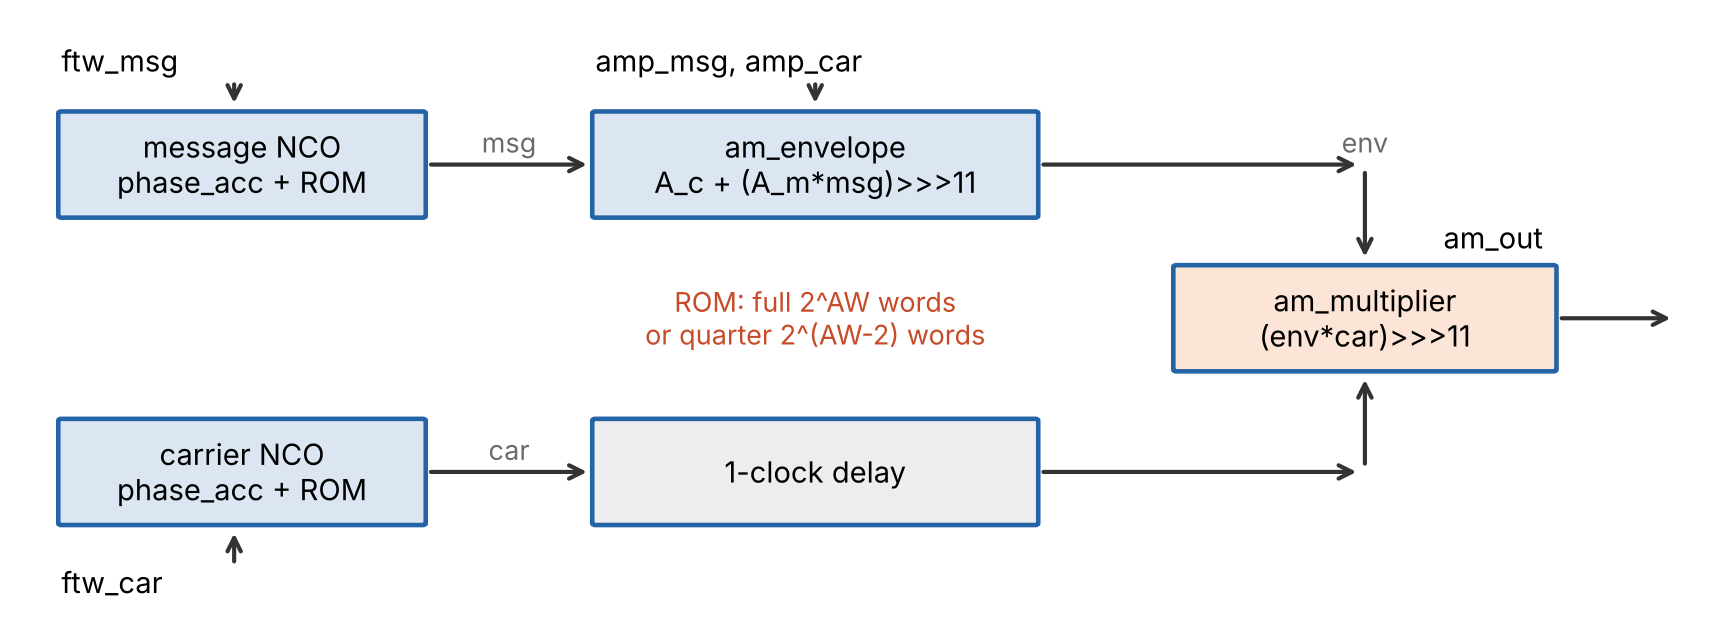
\includegraphics[width=0.78\textwidth]{block_diagram.png}
\caption{Block diagram of the AM modulator. The carrier is delayed by one clock
so that it reaches the multiplier in the same cycle as the registered envelope.}
\label{fig:block}
\end{figure*}

Both ROMs have exactly two register stages, so the NCO latency is identical.
The quarter-wave ROM inverts the address bits when phase bit $AW-2$ is set,
registers the magnitude and, in parallel, the sign bit $AW-1$, and negates the
registered magnitude in the second stage. The carrier is delayed by one
register before the multiplier to match the registered envelope, so the output
appears three clock cycles after the phase accumulators.

\begin{table}[t]
\caption{Datapath widths.}
\label{tab:widths}
\centering
\small
\begin{tabular}{@{}lccc@{}}
\toprule
Operation & Inputs (bits) & Raw product & After shift\\
\midrule
$A_m\cdot m$ & 12 $\times$ 12 & 25 & 14\\
$e\cdot c$   & 14 $\times$ 12 & 26 & 16\\
\bottomrule
\end{tabular}
\end{table}

The unsigned amplitude $A_m$ is extended with a leading zero and declared signed
before the multiplication, so the product is correct in the negative half of
the message.

\section{Verification}
The reference is an integer-only Python model that reproduces
\eqref{eq:fixed} sample by sample. The Verilog testbench reads the stimulus
parameters from the command line and writes the output samples to a text file.
After reset the output starts with three warm-up samples; these are skipped
explicitly and the remaining 10\,000 samples are compared with the model. The
acceptance criterion is bit-exact equality of all 10\,000 samples.

Thirteen configurations are run (Table~\ref{tab:cases}). Cases 1--5 vary $\mu$,
case~6 sets $A_c=0$ (DSB-SC), case~7 raises the message to 100~kHz, and cases
8--13 cross the three address widths with the two ROM architectures at
$\mu=0.5$. In addition, a Hann-windowed FFT of the 10\,000 RTL samples (bin width
10~kHz, so every line falls on an exact bin) is used to check that the output
contains the three lines of \eqref{eq:lines} at the expected frequencies with
amplitude ratio $\mu/2$, and to measure the SFDR, defined as the strongest
intended line over the largest FFT bin outside the guard bands of the intended
lines, with DC counted as a spur.

\begin{table*}[t]
\caption{Verification results for the 13 configurations (10\,000 samples each; SFDR from a Hann-windowed FFT of the RTL output).}
\label{tab:cases}
\centering
\small
\begin{tabular}{@{}rccrrcccrc@{}}
\toprule
\# & AW & ROM & $A_c$ & $A_m$ & $\mu$ & Envelope range & Output range & Mismatches & SFDR (dB)\\
\midrule
1 & 8 & Full & 2000 & 0 & 0 & 2000\ldots2000 & -2000\ldots1999 & 0 & 48.2\\
2 & 8 & Full & 2000 & 500 & 0.25 & 1500\ldots2499 & -2498\ldots2497 & 0 & 48.1\\
3 & 8 & Full & 2000 & 1000 & 0.5 & 1000\ldots2999 & -2998\ldots2997 & 0 & 48.1\\
4 & 8 & Full & 2000 & 2000 & 1 & 0\ldots3999 & -3997\ldots3996 & 0 & 48.1\\
5 & 8 & Full & 2000 & 3000 & 1.5 & -999\ldots4998 & -4995\ldots4994 & 0 & 48.1\\
6 & 8 & Full & 0 & 1000 & -- & -1000\ldots999 & -1000\ldots999 & 0 & 47.9\\
7 & 8 & Full & 2000 & 1000 & 0.5 & 1000\ldots2999 & -2985\ldots2984 & 0 & 48.1\\
8 & 8 & Full & 2000 & 1000 & 0.5 & 1000\ldots2999 & -2998\ldots2997 & 0 & 48.1\\
9 & 8 & Quarter & 2000 & 1000 & 0.5 & 1000\ldots2999 & -2998\ldots2997 & 0 & 48.1\\
10 & 10 & Full & 2000 & 1000 & 0.5 & 1000\ldots2999 & -2998\ldots2997 & 0 & 60.7\\
11 & 10 & Quarter & 2000 & 1000 & 0.5 & 1000\ldots2999 & -2998\ldots2997 & 0 & 60.7\\
12 & 12 & Full & 2000 & 1000 & 0.5 & 1000\ldots2999 & -2998\ldots2997 & 0 & 71.9\\
13 & 12 & Quarter & 2000 & 1000 & 0.5 & 1000\ldots2999 & -2998\ldots2997 & 0 & 71.9\\
\bottomrule
\end{tabular}
\end{table*}


\section{Results}
\subsection{Bit-exact verification and spectra}
All 13 configurations match the golden model with zero mismatching samples
(Table~\ref{tab:cases}). For the default stimulus ($\mu=0.5$) the envelope runs
from 1000 to 2999 and the output from $-2998$ to $2997$; the output peak lies
one count below $A_c(1+\mu)$ because the right shift truncates toward
$-\infty$. At $\mu=1$ the envelope reaches 0, and at $\mu=1.5$ it goes down to
$-999$: the output keeps the three-line spectrum but the envelope detector
would see the folded envelope of Fig.~\ref{fig:wave}(b).

\begin{figure*}[t]
\centering
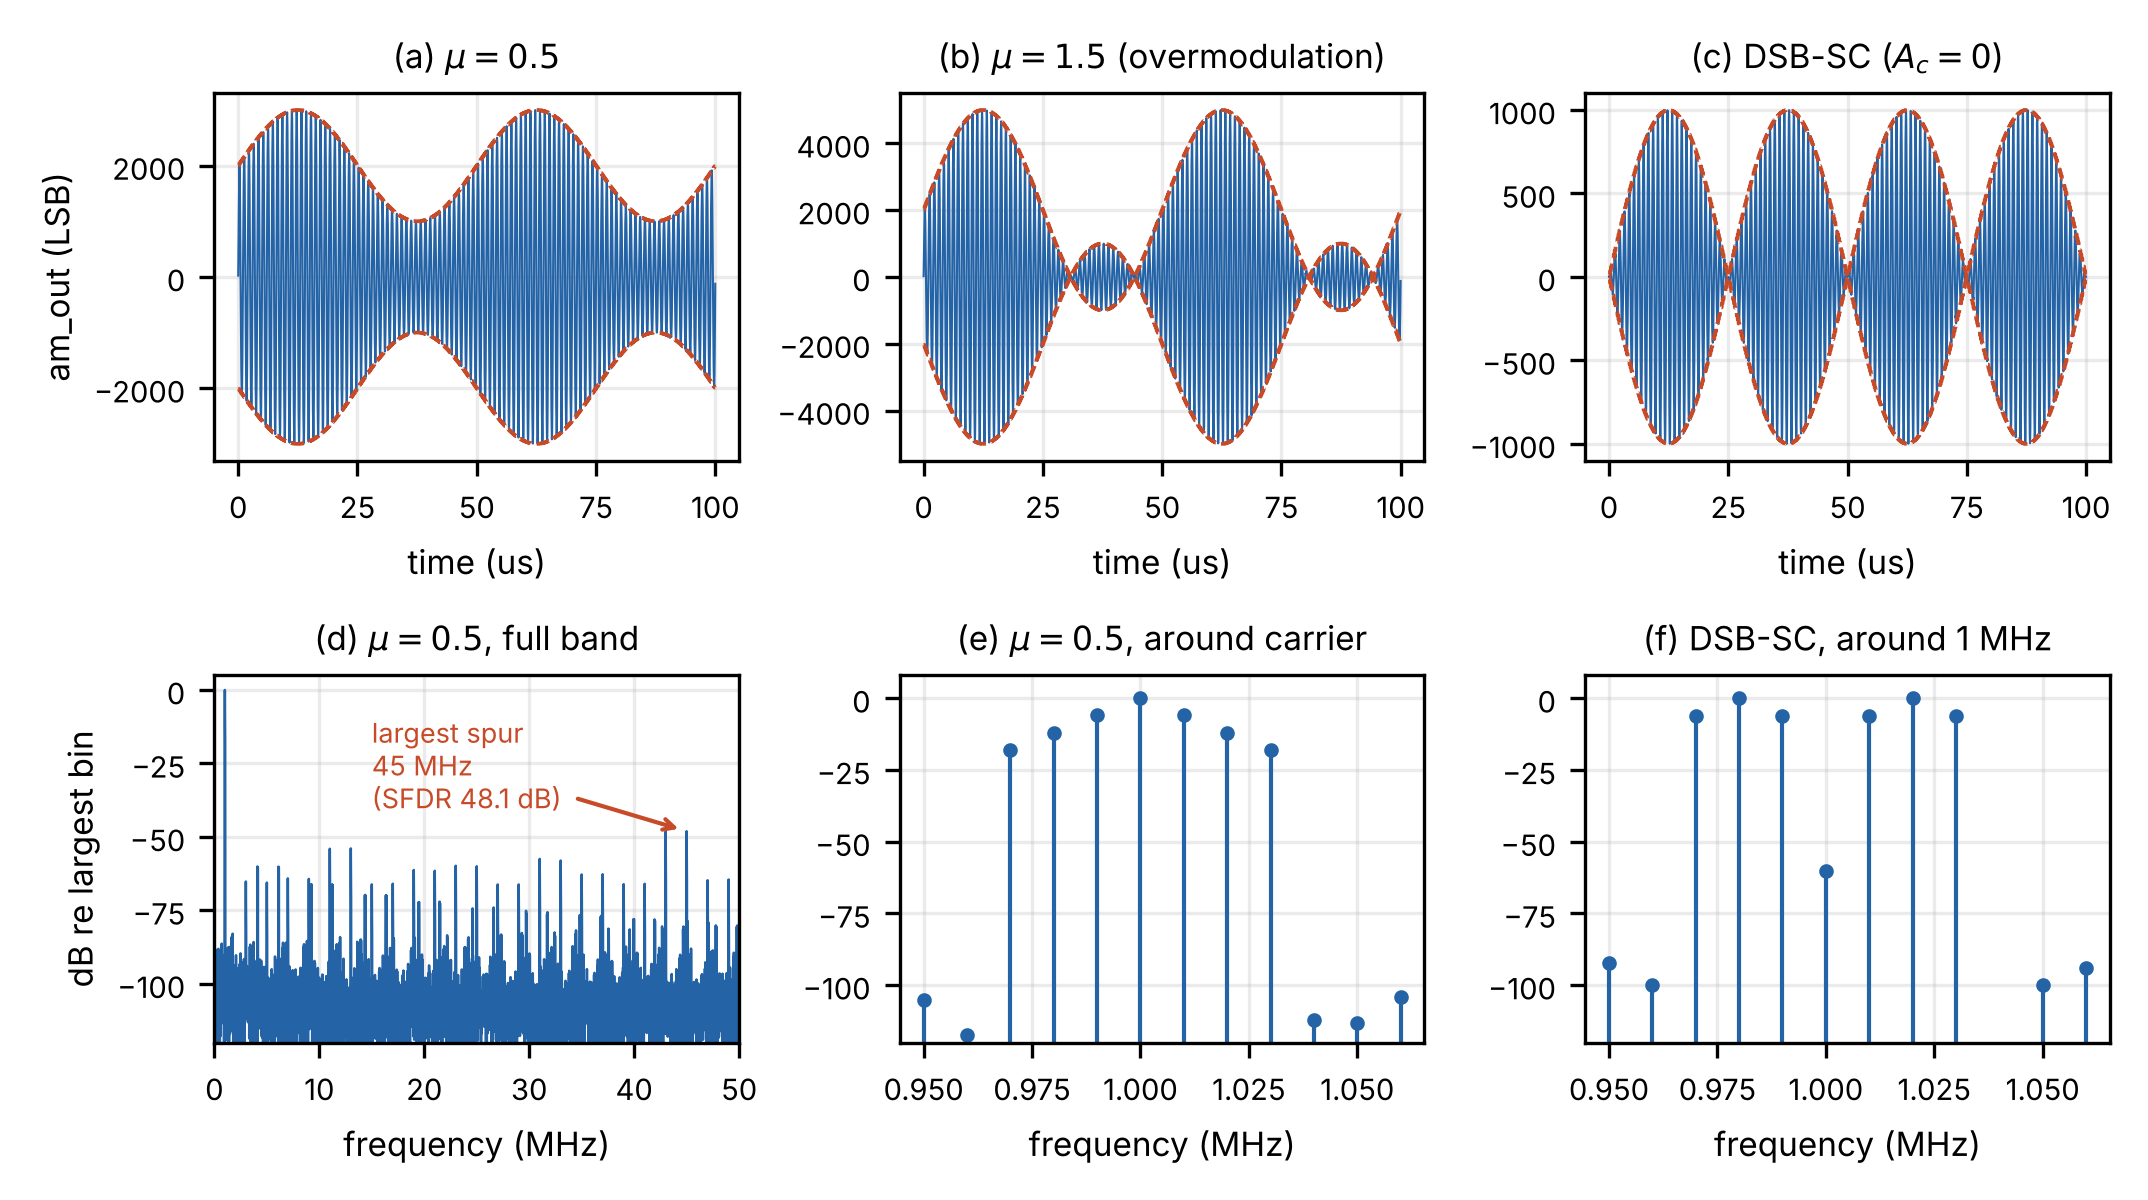
\includegraphics[width=0.92\textwidth]{waveforms_spectra.png}
\caption{RTL output (solid) with the signed envelope (dashed) for (a)~$\mu=0.5$,
(b)~$\mu=1.5$ and (c)~DSB-SC; spectra of the $\mu=0.5$ output over the full band (d)
and around the carrier (e), and of the DSB-SC output (f). Hann window, 10\,000 samples.}
\label{fig:wave}
\end{figure*}

The measured spectrum has the three lines at 980, 1000 and 1020~kHz with no
frequency error at the 10~kHz bin width, and each sideband lies within
$2\times10^{-4}$ of $\mu/2$ times the carrier in every case with a carrier
(Fig.~\ref{fig:wave}(e)). With $A_c=0$ the carrier bin falls 60.1~dB below the
sidebands (Fig.~\ref{fig:wave}(f)), and raising the message to 100~kHz widens the
occupied band to 200~kHz $=2f_m$.

\subsection{Full-cycle versus quarter-wave ROM}
At every address width the full-cycle and quarter-wave designs produce the same
10\,003 output words, so Table~\ref{tab:cases} and Fig.~\ref{fig:sfdr} show a single
SFDR per $AW$: 48.07, 60.72 and 71.88~dB for $AW=8$, 10 and 12, against
$6.02\,AW=48.2$, 60.2 and 72.2~dB. The largest spur lies at 45, 25 and 3~MHz
respectively, far from the three AM lines. The quarter-wave table needs 768, 3\,072
and 12\,288 bits instead of 3\,072, 12\,288 and 49\,152.

\begin{figure*}[t]
\centering
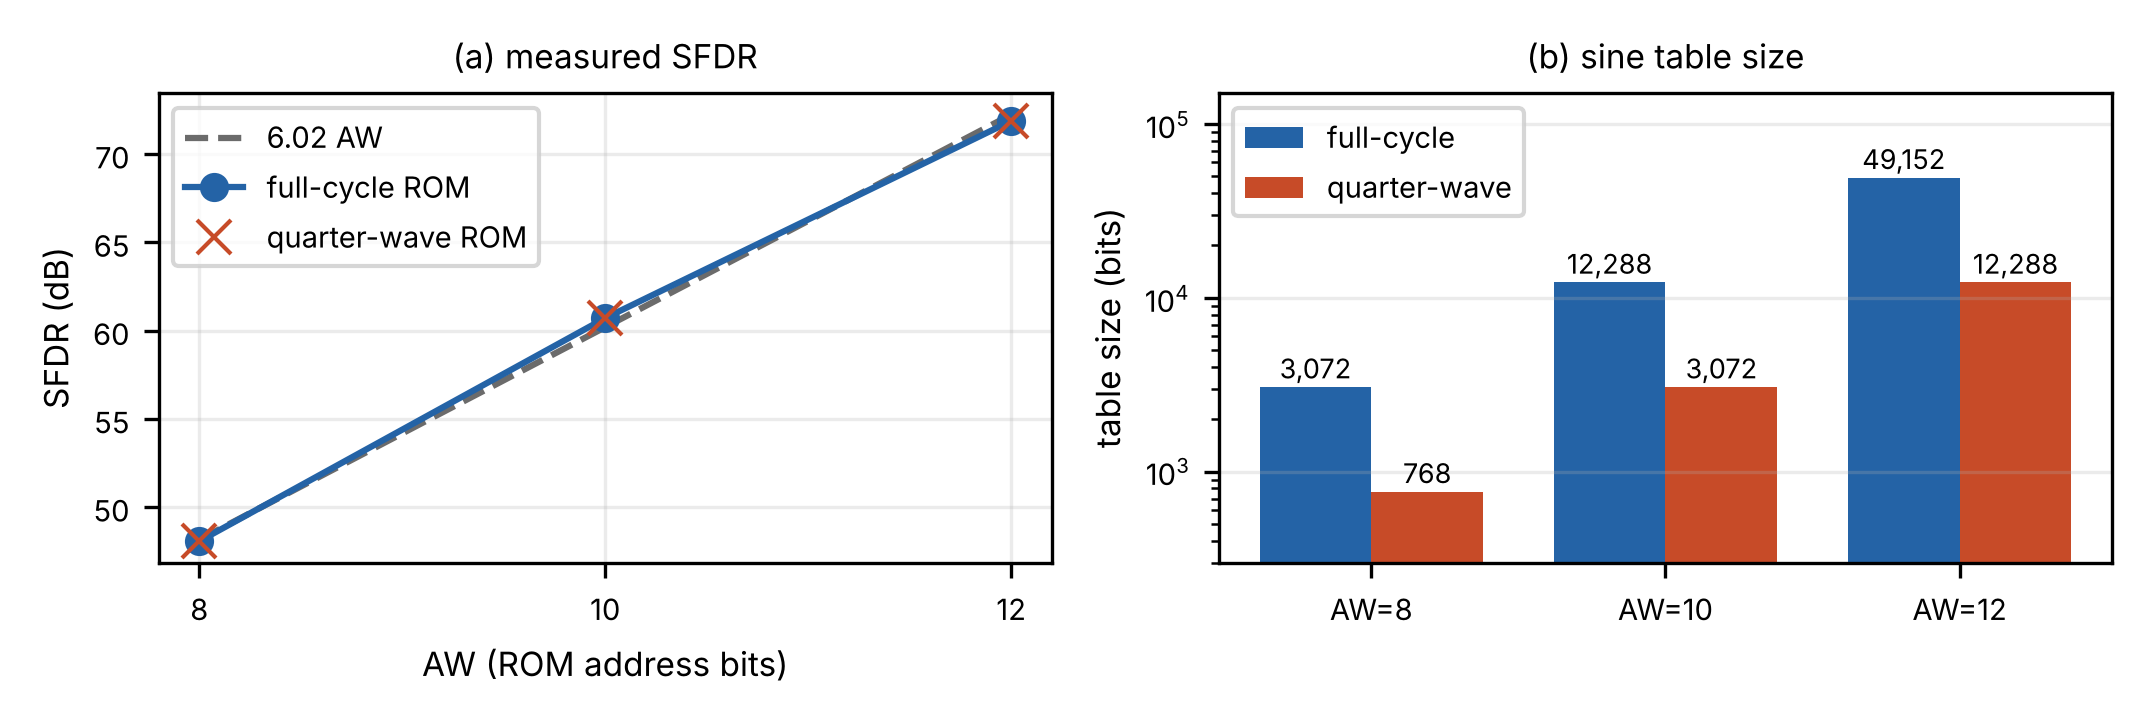
\includegraphics[width=0.92\textwidth]{sfdr_and_memory.png}
\caption{(a)~SFDR versus address width $AW$; the quarter-wave points coincide with
the full-cycle points. (b)~Sine table size.}
\label{fig:sfdr}
\end{figure*}

\subsection{Resources, timing and power}
Table~\ref{tab:res} lists the post-implementation results. Each row is traceable to
\texttt{results/rpt/AW<aw>\_<arch>/}.

\begin{table*}[t]
\caption{Post-implementation results, xc7a35tcpg236-1, 100~MHz target (out-of-context). $F_{max}=1/(10\,\mathrm{ns}-\mathrm{WNS})$.}
\label{tab:res}
\centering
\small
\begin{tabular}{@{}clrrrrrrrrr@{}}
\toprule
AW & ROM & Table bits & LUT & FF & LUTRAM & BRAM & DSP & WNS (ns) & $F_{max}$ (MHz) & $P_{dyn}$ (W)\\
\midrule
8 & Full & 3\,072 & -- & -- & -- & -- & -- & -- & -- & --\\
8 & Quarter & 768 & -- & -- & -- & -- & -- & -- & -- & --\\
10 & Full & 12\,288 & -- & -- & -- & -- & -- & -- & -- & --\\
10 & Quarter & 3\,072 & -- & -- & -- & -- & -- & -- & -- & --\\
12 & Full & 49\,152 & -- & -- & -- & -- & -- & -- & -- & --\\
12 & Quarter & 12\,288 & -- & -- & -- & -- & -- & -- & -- & --\\
\bottomrule
\end{tabular}
\end{table*}


\section{Discussion}
\textbf{Equivalence of the two architectures.} The quarter-wave ROM is a pure
storage optimisation: it reproduces the full-cycle output sample for sample, so
nothing is paid in signal quality, and SFDR is set by the address width alone.
The roughly 6~dB per address bit gain is the price-performance knob; the memory
saving is independent of it, a constant 75\%.

\textbf{Memory versus logic.} \todo{Compare LUT, LUTRAM/BRAM and $F_{max}$ of the
two architectures at $AW=8$, 10 and 12 using Table~\ref{tab:res}: where the fold
logic outweighs the memory saved, and whether the negation shortens the
maximum frequency.}

\textbf{Limitations.} The design has not been run on a board; results are
simulation and Vivado out-of-context implementation. The message is a single
tone. The constraint file defines only the 10~ns clock and sets false paths on all
ports, so $F_{max}=1/(10\,\mathrm{ns}-\mathrm{WNS})$ reflects register-to-register
paths inside the modulator and not I/O timing. Power is the vectorless Vivado
estimate. Each configuration was implemented once with one tool version.

DSB-SC needs no extra hardware: it is the same datapath with $A_c=0$, and it
saves the carrier power at the cost of a coherent demodulator.

\section{Conclusion and Future Work}
A parameterized fixed-point AM modulator was verified bit-exactly against an
integer golden model on 13 configurations, and its two sine-ROM variants were
shown to be output-equivalent at three table sizes while the quarter-wave table
stores 75\% fewer bits. \todo{State the measured LUT, BRAM and $F_{max}$ trade-off.}
Future work includes an envelope detector to close the modulate--demodulate
chain, single-sideband modulation, pipelining to raise $F_{max}$,
switching-activity-based power estimation and an AXI-Stream wrapper for a Zynq
design.

\begin{thebibliography}{9}
\bibitem{tierney1971}
J.~Tierney, C.~M. Rader, and B.~Gold, ``A digital frequency synthesizer,''
\emph{IEEE Trans. Audio Electroacoust.}, vol.~AU-19, no.~1, pp.~48--57, Mar. 1971.

\bibitem{nicholas1987}
H.~T. Nicholas III and H.~Samueli, ``An analysis of the output spectrum of direct
digital frequency synthesizers in the presence of phase-accumulator truncation,''
in \emph{Proc. 41st Annu. Freq. Control Symp.}, 1987, pp.~495--502.

\bibitem{vankka2005}
J.~Vankka, \emph{Digital Synthesizers and Transmitters for Software Radio}.
Dordrecht, The Netherlands: Springer, 2005.

\bibitem{haykin2001}
S.~Haykin, \emph{Communication Systems}, 4th ed. New York, NY, USA: Wiley, 2001.

\end{thebibliography}

\end{document}
